\documentclass[12pt]{article}
\usepackage{geometry}
\usepackage{xcolor}
\usepackage{hyperref}
\usepackage[utf8]{inputenc}
\usepackage{tabto}
\usepackage{graphicx}
\usepackage{biblatex}
\usepackage{pdflscape}
\addbibresource{bibliography.bib}
\graphicspath{ {./images/} }
\hypersetup{
colorlinks=false,
linktoc=all
}
\geometry{
a4paper,
left=30mm,
top=30mm,
right=30mm,
bottom=40mm
}
\newcommand{\black}{
\pagecolor{black}
\color{white}
}
\newcommand{\sentence}{} % New sentence
\newcommand{\final}{} % Mark a section as finished
\newcommand{\italic}[1]{\textit{#1}}
\title{Vectorization and Compression of Animated Cartoon Videos}
\author{Bassam Helal}
\date{September 2020}
\begin{document}
    % TODO 12-Sep-20 Remove black background and white text
    \black

    \pagenumbering{gobble} % Remove page numbering

    \maketitle

    \begin{center}
        \vspace{8cm}
        
\includegraphics[scale=0.65]{SwanseaUniversityLogo.png}
    \end{center}

    \pagebreak

    \begin{center}
        \section*{Abstract}
    \end{center}

    % TODO 12-Sep-20 Abstract

    \pagebreak

    \renewcommand*\contentsname{
    \begin{center}
        Table of Contents
    \end{center}}

    \tableofcontents

    \pagebreak

    \pagenumbering{arabic} % Begin page numbering from here


    \section{Introduction}\label{sec:introduction}

    % A paragraph or so for each of:

    % Project Description
    % Motivation
    % Existing Literature
    % Limitations of the literature that we will attempt to tackle
    % Aims and Objectives
    % Discoveries and results we found after our attempts
    % Section Signposting

    \pagebreak


    \section{Background}\label{sec:background}

    \tab
    This document makes no assumption of the reader's knowledge in computer graphics and its related fields,
    thus, this section will introduce the reader to some of the required knowledge needed for understanding this
    project.
    \sentence
    Firstly, we will introduce raster graphics, ie, the current common standard for graphics data representation.
    We will then introduce its counterpart vector graphics, a different way to store graphics data that is growing in
    popularity and has its own advantages and disadvantages.
    \sentence
    We will then give a brief primer on image compression and some common methods of reducing the overall size
    of an image.
    \sentence
    Finally, we will explain how this all ties into video graphics and describe some of the few differences between
    image graphics and video graphics.

    \subsection{Raster Graphics}\label{subsec:raster-graphics}

    % 1 - 2 sentences for each of:
    % Brief summary of what we will go over (signposting)
    % Pixels, Bitmaps, Image Data Buffers: basically the bare must knows about Raster Graphics
    % Advantages and popularity of Raster Graphics
    % Disadvantages like upscaling, pixelation, size issues with high resolution
    % Brief summary of everything we just mentioned

    \tab
    Raster graphics is the current most popular way of representing and storing graphics data.
    \sentence
    This representation format stores the image data as a grid of pixels, a pixel (picture element) being the color
    of the image at a particular point in the grid.
    \sentence
    Colors can be represented in a variety of ways but the most common is RGB with RGBA also being found in some
    formats.
    \sentence
    Each channel has a bit depth which details the number of possible colors that the channel can contain with 8 bits
    per channel being the current most common but higher values exist as well such as 10 and 12 bits per channel.
    \sentence
    Thus the image data is a 2 dimensional array of pixels which could be 3 or 4 channels of 8 bit values, thus an
    image can also be represented as a 3 dimensional array with the last dimension being 3 or 4 values in size
    representing the 3 or 4 channels of that pixel.
    \sentence
    The resolution of an image is the number of pixels it contains, which is the image's width multiplied by its
    height, higher resolution images have more detail but are also more expensive to store as there is more data.
    \sentence
    Raster graphics are the most popular form of image and generally graphics representation, they allow for easy
    representation and computationally cheap as well since all the data is stored with no extra work needed.
    \sentence
    The main disadvantages of raster graphics have to with image resolution and detail, namely that images will show
    pixelation artifacts when they are displayed at a higher resolution than they are actually stored at, thus the
    image appears to show the raw pixels.
    \sentence
    % TODO 16-Sep-20 Show pixelation images
    To compensate for this, higher and higher resolution images are needed but those come at the cost of size.
    \sentence
    % TODO 16-Sep-20 Explain more about raw size (no compression, so use raw format or just plain numbers)
    \sentence
    % TODO 16-Sep-20 Summarize

    \subsection{Vector Graphics}\label{subsec:vector-graphics}

    % 1 - 2 sentences for each of:
    % Brief summary of what we will go over (signposting)
    % Declarative vs Imperative ie WYSIWYG vs WYSIWYM, describing the image using primitive geometry
    % Advantages of Vector especially in contrast to Raster (size and scalability), mention uses and popularity
    % Disadvantages like portability and light technical stuff like gradients and photographs
    % Brief summary of everything we just mentioned

    % TODO 16-Sep-20 We can make a small table comparing Raster & Vector Graphics for the attributes like size,scalability etc

    \subsection{Image Compression}\label{subsec:image-compression}

    % 1 - 2 sentences for each of:
    % Brief summary of what we will go over (signposting)
    % Fundamentals of Compression (type-agnostic) things like compression rate and lossy-ness or accuracy
    % Lossless Image Compression (PNG, BMP etc)
    % Lossy Image Compression (JPEG, GIF etc)
    % Brief summary of everything we just mentioned

    % TODO 16-Sep-20 We can have an image comparing popular image file types with regards to compression

    \subsection{Video Graphics}\label{subsec:video-graphics}

    % 1 - 2 sentences for each of:
    % Brief summary of what we will go over (signposting)
    % How video is stored and how it relates to Images (mostly the same)
    % Common file types and how they compress and store video data (MP4, MKV, H265 etc)
    % Evidence and proof of why video is expensive (and also popular)
    % Brief summary of everything we just mentioned

    \subsection{Toolchain}\label{subsec:toolchain}

    % 1 - 2 sentences for each of:
    % Brief summary of what we will go over (signposting)
    % Node.js
    % JavaScript, TypeScript (benefits over JS)
    % Supplementaries like Electron, GPU.js, OpenCV etc
    % Brief summary of everything we just mentioned

    % TODO 19-Sep-20 Shorten!
    \tab
    This project uses a variety of popular tools and libraries to achieve its aims and objectives both efficiently
    and quickly, this section will briefly go over the most important tools used.
    \sentence
    This project uses Node.js as its runtime platform, Node.js is a cross-platform runtime environment that executes
    JavaScript code on a machine instead of the usual JavaScript runtime, the browser.
    \sentence
    The choice for Node.js was made paradoxically because of both a familiarity with the runtime and the JavaScript
    ecosystem as well as a strong desire to further enhance our knowledge and experience in both the platform and
    ecosystem.
    \sentence
    Node.js allows us to access the ever-growing JavaScript ecosystem which includes very powerful libraries and
    frameworks for both front-end designs and back-end computationally heavy workloads.
    \sentence
    Node.js uses JavaScript as its runtime language, while JavaScript is a powerful and excellent language for
    rapid-prototyping, it is also a very error-prone language as it has no typing checks in place.
    \sentence
    TypeScript is a programming language that is a strict superset of JavaScript that adds typing features onto
    JavaScript and transpiles to performant, cross-platform compatible JavaScript by means of a TypeScript compiler.
    \sentence
    TypeScript was chosen as the programming language of choice for the project for its many benefits not limited to
    its added type safety.
    \sentence
    The JavaScript ecosystem provides us with some powerful libraries and frameworks for application development,
    this project makes use of some excellent noteworthy tools such as Electron, GPU.js and OpenCV among other tools.
    \sentence
    Electron allows developers to write desktop applications using web technologies, it essentially is a Chromium
    browser with two processes, a front-end process(es) called the "renderer" which is similar to a Chromium web page
    that displays HTML, and a back-end process called the main process which is a Node.js process.
    \sentence
    Electron combines Node.js and Chromium to allow a developer to write a native desktop application using the same
    technologies used on the web, this has its own advantages and disadvantages but in our case, it means we can
    quickly develop a GUI desktop application that can access our Node.js code without resorting to web servers and
    other more complicated means.
    \sentence
    GPU.js is a JavaScript library that allows developers to run code on the host machine's GPU making use of the
    GPGPU (General-Purpose computing on Graphics Processing Units) paradigmGeneral-purpose computing on graphics
    processing units.
    \sentence
    This can allow for very large performance improvements and speedups for computationally expensive mathematical
    computations.
    \sentence
    % TODO 19-Sep-20 OpenCV? We didn't use it too much and this is already getting too long
    \sentence
    In summary, the project uses the Node.js runtime for its large ecosystem, the TypeScript programming language for
    its added type safety benefits, Electron to easily display a GUI and GPU.js to run code on the GPU for additional
    performance when needed.
    \pagebreak


    \section{Related Work}\label{sec:related-work}

    % Here we throw a lot of the current stuff from both research and industry and show their flaws and limitations
    % (which we may or may not have tackled)

    \subsection{Current Research}\label{subsec:current-research}

    % Brief summary of what we will go over (signposting)
    % New Machine Learning methods for Vectorization
    % New Machine Learning methods for Compression
    % Novel approaches and ideas within Vectorization such as mesh gradients etc (no ML)
    % Brief summary of everything we just mentioned

    \subsection{Current Applications}\label{subsec:current-applications}

    % Brief summary of what we will go over (signposting)
    % Adobe Illustrator, Logos, Topography, Medical stuff like X rays etc Potrace
    % Animations and Games using Vector as the development method
    % Current Image \& Video compression algorithms such as PNG, H265 and H266 (no ML)
    % Brief summary of everything we just mentioned

    \subsection{Limitations}\label{subsec:limitations}

    % Brief summary of what we will go over (signposting)
    % Why ML is absolute hot trash
    % Show off the flaws with existing technologies while showing how we tackled (and hopefully beat) them
    % Discuss inherent limitations of this process, such as issues with Vector Graphics and input data being varying etc
    % Brief summary of everything we just mentioned

    \pagebreak


    \section{Implementation}\label{sec:implementation}

    %  This may get long and technical, we should try to keep things fairly high level as much as
    %  possible we will also show both Math, pseudocode and pipeline of the overall process and avoid boring low level
    %  details

    \subsection{Pipeline}\label{subsec:pipeline}

    \bigskip

    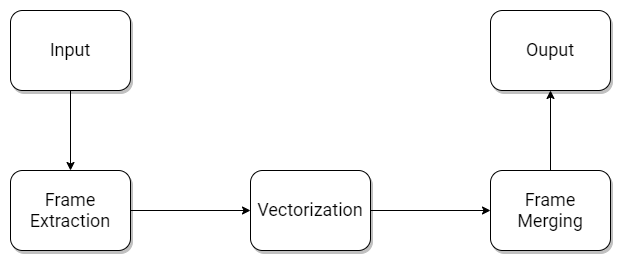
\includegraphics[width=\textwidth]{Pipeline.png}

    % TODO 15-Sep-20 Add a caption, read more here https://cs.overleaf.com/learn/latex/Inserting_Images

    \bigskip

    The above image shows the high level process pipeline of the project from input to output with each phase of the
    pipeline further detailed in its own section below.
    \sentence
    Firstly, we explain the expected input video and its ideal characteristics that will result in a higher accuracy output.
    \sentence
    Then, the first phase of the processing begins, the frame extraction, where the frames of the video are
    extracted to be used further down the pipeline.
    \sentence
    Next, the main phase of the processing, the vectorization of a single frame, we describe and detail the multiple methods
    and approaches that were used in order to gain the highest level of accuracy and compression rate on each frame.
    \sentence
    The final stage of the processing, frame merging combines the vectorized frames back into a playable video form
    with additional computation executed to add favorable traits such as lower file sizes.
    \sentence
    Finally, we explain the output that the process will produce and what an ideal output will be like, particularly in
    comparison to the input file.

    \subsubsection{Input}\label{subsubsec:input}

    % TODO 20-Sep-20 Mention the limitations of Vector and Vectorization somewhere, currently its in 3.3 Limitations
    % but it may be suitable elsewhere

    % Low or no use of gradients so it has discrete colors
    % Fewer and larger color regions, this is why photos are more difficult in addition to gradients
    % Low or no noise
    % No 3D stuff like shadows and reflections

    % TODO 20-Sep-20 Show examples of good cartoons and have images, so Fairly OddParents, Teen Titans Go
    % TODO 20-Sep-20 Show example of some less optimal cartoons like old Tom and Jerry, Hannah Barbera and Ed, Edd n Eddy

    \tab
    First, it is important to understand the input that the process will be expecting and detail what makes an ideal
    input file.
    \sentence
    The minimum requirement is that the input file be a video in any popular format, specifically, one that Ffmpeg
    can use (so basically all formats), however, this project specifically aims to work on animated cartoons so while
    any video will technically work, for the purpose of this project, a video of an animated cartoon is expected.
    \sentence
    However, not all animated cartoons are equal, in fact there is a great deal of variation between cartoons in
    terms of art style, animation method, and many other artistic effects that can heavily influence the output of
    the process.
    \sentence
    Thus, we must define the "ideal" input file, or more precisely, the input file that will produce the best results
    because the process was designed with those files in mind for reasons to do with the limitations of vectorization.
    \sentence
    The ideal input video is one that is most friendly towards vectorization, meaning it has the most vectorizable
    qualities and characteristics with as few incompatibilities as possible, these were mentioned in depth
    in the~\nameref{subsec:limitations} section but will be briefly repeated within this new context.
    \sentence
    Since vectorization is heavily dependent on the color variation of the original raster image, an ideal input
    image would be one with discrete color regions made up of a single color, with no noise, gradients, shadows,
    lighting or any other effects, essentially an image made of a set if color blocks that are very discrete from one
    another.
    \sentence
    In addition to this, it is important to note that we are dealing with moving pictures and it is also ideal to
    have as little noise as possible between frames, this can be an artifact of compression or signal interference
    but can also be seen as an artistic style choice as shown in Cartoon Network's \italic{Ed, Edd n Eddy}.
    \sentence
    Obviously very few real world media is like this, but a surprising number of cartoon videos can come very close
    to this description, with very few complications such as shadows and light gradients.
    \sentence
    An example of a real world cartoon that has these ideal qualities is Nickelodeon's \italic{The Fairly OddParents}
    which uses discrete color regions, very few (if any) gradients and no complex shadows or lighting and thus can be
    described as being a truly 2D cartoon.
    \sentence
    On the other extreme end cartoons with heavy use of photographs and heavy noise are the least ideal as well as
    any 3D cartoons, ie those that make use of 3D effects such as shadows, lighting and many complex gradients.
    \sentence
    Examples include Hanna Barbera cartoons prominent from the 1960s to the 1980s such as \italic{Top Cat} and
    \italic{The Flinstones}, \italic{Looney Tunes} cartoons as well as modern 3D animations such as Pixar Animation
    Studios' \italic{Toy Story} and \italic{The Incredibles}.
    \sentence
    In summary, the minimum required input is simply any video but the expectation is that it will be a video of an
    animated cartoon and the ideal input is a video of an animated cartoon that has highly vectorizable qualities.

    \subsubsection{Frame Extraction}\label{subsubsec:frame-extraction}

    \tab
    The frame extraction phase has a single purpose and that is to convert the input video into a some form of medium
    that can be vectorized, namely images.
    \sentence
    Since the input video will always be frame based, we can thus convert a video into a set of vectorizable units
    that accurately represent its data, frames.
    \sentence
    Each frame of the video will be represented in an image which we can then vectorize in the next step.
    \sentence
    To do this, we use the industry standard tool, Ffmpeg to create a directory of PNG images for each frame of the
    video using the command:
    \begin{verbatim}ffmpeg -i input.mp4 outputDirectory/%d.png -y
    \end{verbatim}
    \sentence
    This is so that the next step (vectorization) can be done on each frame can be independently and can more easily
    be parallelized, since the vectorization of a single frame does not depend on any other frames around it.
    \sentence
    While in theory one can skip this step and read each frame of the video performing the vectorization step in
    serial for each frame, it is much more efficient to split the workload first by first dividing the video into
    frames stored on disk and then perform the vectorization step, now with the additional benefit of being able to
    run the vectorization step on multiple frames at once.

    % TODO 20-Sep-20 Picture?

    \subsubsection{Vectorization}\label{subsubsec:vectorization}

    % Conversion of each Frame to an SVG which will have a single SVG Path element for each color

    \subsubsection{Frame Merging}\label{subsubsec:frame-merging}

    % SVG Frame Joining which will have some smart compression built-in

    \subsubsection{Output}\label{subsubsec:output}

    % An SVG Video that is of course highly scalable and has a lower size than the original if upscaled and with
    % very minimal data loss

    \subsection{Vectorization Methods}\label{subsec:vectorization-methods}

    % Here we will explain our story of the last few months, the many approaches and their failures. This section
    % should implicitly show the reader that the problem is very hard, harder than initially thought to be. If
    % we show the difficulty and the struggle it can explain any poor results and can further show overall contribution
    % that we tried something difficult

    \subsubsection{Color Quantization Approach}\label{subsubsec:color-quantization-approach}

    % From the general process of the library ImageTracer.js

    % Explain Color Quantization
    % Advantages (very accurate, fast, good for logos and web based stuff)
    % Disadvantages (Too dependent on quantization number of colors, large size and poor speed with high number of
    % colors)
    % Show pictures of original vs some different results from this approach (to show why it fails)

    \subsubsection{Connected Component Labelling (CCL)}\label{subsubsec:connected-component-labelling-(ccl)}

    % Using Connected Component Labelling (CCL) to create discrete but adjacent components

    % Explain CCL
    % Reasoning behind approach
    % Possible disadvantages
    % Signpost for the following approaches

    \subsubsection{Edge Based CCL Approach}\label{subsubsec:edge-based-ccl-approach}

    % Using OpenCV Canny Edge detection

    % Explain OpenCV and Canny Edge Detection
    % Reasoning behind approach (edges should form polygons which will be color regions) and the expected result
    % Advantages (fast, easy, accurate for edge detection)
    % Disadvantages (not all edges form polygons and 1 pixel incorrect can have huge effects)

    \subsubsection{Pixel Based CCL Approach}\label{subsubsec:pixel-based-ccl-approach}

    % Using the color of each pixel to form regions with close enough or similar colors

    % Explain pixel data (RGBA) and what it means to be close to a neighboring pixel
    % Reasoning behind approach (an image can be a partition of several color regions)
    % Advantages (surprisingly accurate, little data loss, huge size savings)
    % Disadvantages (slow, complex, Anti-Aliasing and noise affects result so too many 1 pixel regions)

    \subsection{Limitations and Drawbacks}\label{subsec:limitations-and-drawbacks}

    % Here we explain the overall limitations of all the processes we used and really any future process because
    % of the nature of Vectorization of Raster data

    % Brief summary of what we will go over (signposting)
    % Speed or performance (never realtime and requires HPC on GPUs for good speeds) and optimizations required
    % Lossy-ness, the transformation of Raster to Vector is by nature lossy because we are undoing Rasterization
    % artifacts
    % Size, this can be an issue for low resolution images or for very complex images, rasterization is often better
    % Brief summary of everything we just mentioned


    \pagebreak


    \section{Software Engineering}\label{sec:software-engineering}

    \tab
    This section will detail the software engineering aspects of the project's development, specifically the
    methodology used to develop, the risks of the project and the software testing techniques used in the project's
    development.

    % Just the SE stuff and how we applied it during development, briefly mention the changes Covid did to the development

    \subsection{Methodology}\label{subsec:methodology}

    % Extreme Lean Agile because life is unknown beyond 2 days in these strange times we live in :/
    % Here we can show how the poor results affected our schedule and how things shifted because of unexpected results,
    % we can definitely show that this is common in real life and is a good representation and preparation of the real world
    % which has unexpected delays and poor results all the time and how we overcame it all (less sleep and more coffee :D)

    \tab
    The software methodology used for the development of this project is a very lean agile methodology aptly named,
    Lean-Agile.
    \sentence
    % TODO 20-Sep-20 Ref https://www.bluefruit.co.uk/lean-agile-series/whats-lean-agile-how-can-help-you-avoid-project-waste/
    This methodology inherits heavily from modern agile methodologies following all the core principles and values
    but adds principles adapted from lean manufacturing, particularly emphasizing minimal waste and minimal
    prediction.
    \sentence
    While a more commonly known methodology such as Scrum could have been used, it seemed more appropriate to use a
    methodology that has extreme unpredictability built into it nature especially during the growth phase of the
    COVID-19 pandemic, which caused many unpredictable events.
    \sentence
    The pandemic's potentially adverse effects on the development of the project meant that it was critical to use a
    methodology that is extremely efficient and has little fixed planning with a very easy way of adapting to changes.
    \sentence
    This proved to be extremely beneficial, more so than expected because of the many major roadblocks that were
    faced during development which are further explained in detail in the~\nameref{sec:results-and-findings} section.
    \sentence
    The constant occurrence of very negative results, especially after a complex and time-consuming amount of work
    put in meant that plans had to change and adapt rapidly in accordance to this, which is common and expected in
    any research based project such as this one.
    \sentence
    As a result, while the Lean-Agile methodology is an unorthodox methodology choice, it was absolutely the correct
    one to use and has been the saving grace of the time management of this project since very few other
    methodologies could have allowed for the rapid adaptation and movement of this project.

    \subsection{Schedule}\label{subsec:schedule}

    % Followed it well but started falling apart towards the end, very accurate to the real world :D
    % Mention that we started dissertation somewhat early to avoid the risk of running out of time

    \tab
    While the Lean-Agile methodology is not particularly well suited to long term predictions, it is still important
    to have a schedule in place in order to keep track of time and to have a general idea of how many tasks are left
    and how much time is available to complete them, even if the predictions of time may be incorrect.
    \sentence
    This is why a Gantt Chart was used to plot a schedule containing the general phases of the project's development
    against the time allocated to work on the project.
    \sentence
    % TODO 21-Sep-20 Describe what is a Gantt Chart
    \sentence
    % TODO 21-Sep-20 Introduce the Gantt chart below


    \pagebreak
    \thispagestyle{empty}
    \begin{landscape}
        \begin{center}
            \huge{Gantt Chart}
        \end{center}
    \end{landscape}
    \pagebreak

    % TODO 21-Sep-20 Detail the stuff we showed in the chart above

    \pagebreak

    \subsection{Risks}\label{subsec:risks}

    \tab
    Naturally, a project of this scale that is very experimental in nature has many multi-faceted risks
    associated with it that can severely impact the development of the project if not correctly mitigated.
    \sentence
    As such, it is important to detect these risks as early as possible and have detailed and usable mitigation
    strategies to counter such risks and avoid their possibly devastating effects.
    \sentence
    % TODO 21-Sep-20 Introduce the chart below and describe the format of the chart
    % TODO 21-Sep-20 Chart should have Risk name, description, type? Probability, Consequentiality, mitigation

    \pagebreak
    \thispagestyle{empty}
    \begin{landscape}
        \begin{center}
            \huge{Risks Chart}
        \end{center}
    \end{landscape}
    \pagebreak

    \subsection{Testing}\label{subsec:testing}

    % Short and quick, show some basic testing stuff
    % Unit Testing for accuracy and of course Manual Acceptance testing (to ensure images actually open, are not corrupt etc)

    \pagebreak


    \section{Evaluation}\label{sec:evaluation}

    % Two main angles, accuracy to the original and compression rate from the original
    % As much as possible we need to emphasize that we have done something great,
    % no lying, just selective and sometimes exaggerated benchmarks in order to further our claim that we
    % have accomplished something meaningful

    \subsection{Accuracy}\label{subsec:accuracy}

    % Define accuracy (aka lossy-ness or how much data is lost from original)
    % Quantitative methods (compare each pixel to itself), and compare with other compression methods like JPEG
    % Qualitative methods (human eye side by side) and compare with other methods like JPEG

    \subsection{Compression}\label{subsec:compression}

    % Define compression rate (aka how smaller is the result compared to original or some other)
    % Quantitative methods (compare against original, AND against others including upscaled and uncompressed)
    % Qualitative methods (file transfer speeds of smaller sizes and how smaller files are better for users)

    \pagebreak


    \section{Results and Findings}\label{sec:results-and-findings}

    % Here we show both the results of our development but also our own personal findings that someone who
    % wants to research this kind of thing should be aware of that I discovered

    \subsection{Results}\label{subsec:results}

    % The good, the bad and the ugly (with detailed explanations :D)

    \subsection{Findings}\label{subsec:findings}

    % This is a very difficult problem, more difficult than initially thought to be
    % GPU acceleration is very hard but improves speed shockingly well
    % Node sucks for concurrency and doesn't have true multi-threading
    % Differing input will have different results because of the limitations of vectorization

    \pagebreak


    \section{Challenges}\label{sec:challenges}

    \subsection{Toolchain}\label{subsec:toolchain2}

    % Toolchain used was not very mature or helpful sometimes

    \subsection{Performance}\label{subsec:performance}

    % GPU programming is insanely difficult but yields huge benefits (leading to very difficult decisions)
    % Optimizations to increase speed are also difficult and especially so on a non-multi-threaded environment like Node

    \subsection{Minimizing Human Interaction}\label{subsec:minimizing-human-interaction}

    % Reducing the number of human inputted arguments to create a fully autonomous deterministic system that is not
    % ML based and produces very accurate results is very difficult

    \pagebreak


    \section{Reflection}\label{sec:reflection}

    % How would you do it differently if to start from scratch (Use JVM or Native and optimize for GPU early)
    % Project Management (Fairly good given the circumstances)
    % So much new knowledge about many different things
    % Very difficult but very mentally stimulating and rewarding project that I really enjoyed

    \pagebreak


    \section{Future Work}\label{sec:future-work}

    % Use better tools that allow for native multi-threading and easier and direct access to GPU
    % Better optimizations and better compression
    % Explore having a mixed raster and vector solution to solve the areas where vector fails
    % Buy better hardware for faster development :D

    \pagebreak


    \section{Conclusion}\label{sec:conclusion}

    % Summarize everything we said
    % Conclude with final thoughts about the good, the bad and how this can further improve the world etc

    \pagebreak


    \printbibliography[heading=bibintoc,title={References}]

    \pagebreak

\end{document}